\documentclass[11pt]{article}
\usepackage[margin=1in]{geometry}
\usepackage{amsmath,amssymb,booktabs,graphicx,setspace,caption,hyperref}
\usepackage[T1]{fontenc}
\usepackage{mathpazo}
\setlength{\parindent}{0pt}
\setlength{\parskip}{0.6em}
\captionsetup{font=small,skip=6pt}
\title{Panel MS-AR(1) with random-effects intercepts, full sample\\[0.4em]\large Real GDP per worker (period-average USD)}
\author{}
\date{}
\begin{document}
\maketitle
\section{Model}
Joint panel Markov-switching AR(1) around a \emph{linear} trend, with three regimes:
\begin{align}
y_{it} &= a_i + g\, t + z_{it}, \\
z_{i,t+1} &= \bigl(1-\rho(s_{it})\bigr)\mu(s_{it}) + \rho(s_{it})\, z_{it} + \sigma(s_{it})\,\varepsilon_{it}, \\
s_{i,t+1} &\sim \Pi(\,\cdot\mid s_{it}), \\
a_i &\sim \mathcal{N}(\alpha,\omega^2) \quad \text{(random effects)}.
\end{align}
The outcome is log real GDP per worker (period-average USD) from the 2026-09-11 quarterly panel. Calendar time is taken from the period stamp $t$ (year-fraction). The trend is linear in calendar time $t$ ($g$ per year, common across countries). In the pooled specification $a_i\equiv a$. In the random-effects specification the $a_i$ are i.i.d.\ Normal draws; $\alpha$ and $\omega$ are estimated by maximum likelihood, integrating each country's Hamilton-filter likelihood by 11-point Gauss--Hermite quadrature. Cycles are plotted using the posterior mean of $a_i$. Latent paths $s_{it}$ are country-specific. The regime dated $t$ governs the transition from $z_t$ to $z_{t+1}$. $\sigma$ and $\rho$ switch with the regime. The median $\mu$ is pinned at 0. $|\rho|<0.99$.
Standard errors (in parentheses) are delta-method from a numerical Hessian on shared parameters. $\pi$ is the ergodic distribution of $\Pi$. $E[z]$ is the long-run mean of the cycle implied by $\mu$, $\rho$, and $\Pi$.
\clearpage
\section{Common intercept and linear trend}
2026-09-11 panel, full sample: log real GDP per worker. 95 countries, 8937 observations, 1963-Q1--2026-Q2. Fitted countries: 95. Observations: 8937. Log-likelihood: 11694.19. Ergodic mean of the cycle $E[z]=0.4891$ (0.0830).
Common intercept $a=-5.7220$ (0.0997). Common slope $g=0.0047$ (0.0018).
\begin{table}[h]
\centering
\caption{Regime AR(1), transition matrix, and ergodic $\pi$. Columns are regimes.}
\begin{tabular}{lccc}
\toprule
 & (0) & (1) & (2) \\
\midrule
$\mu$ & -0.2840 & 0.0000 & 1.3478 \\
 & (0.1097) & --- & (0.0778) \\ \addlinespace
$\sigma$ & 0.0972 & 0.4095 & 0.0403 \\
 & (0.0014) & (0.0161) & (0.0005) \\ \addlinespace
$\rho$ & 0.9900 & 0.6361 & 0.9900 \\
 & (0.0000) & (0.0422) & (0.0000) \\ \addlinespace
$\Pi_{0\cdot}$ & 0.9870 & 0.0018 & 0.0112 \\
 & (0.0021) & (0.0009) & (0.0020) \\ \addlinespace
$\Pi_{1\cdot}$ & 0.0238 & 0.9455 & 0.0307 \\
 & (0.0100) & (0.0125) & (0.0107) \\ \addlinespace
$\Pi_{2\cdot}$ & 0.0084 & 0.0028 & 0.9888 \\
 & (0.0015) & (0.0009) & (0.0015) \\ \addlinespace
$\pi$ & 0.4222 & 0.0417 & 0.5361 \\
 & (0.0377) & (0.0110) & (0.0374) \\ \addlinespace
\bottomrule
\end{tabular}
\end{table}
\begin{figure}[h]
\centering
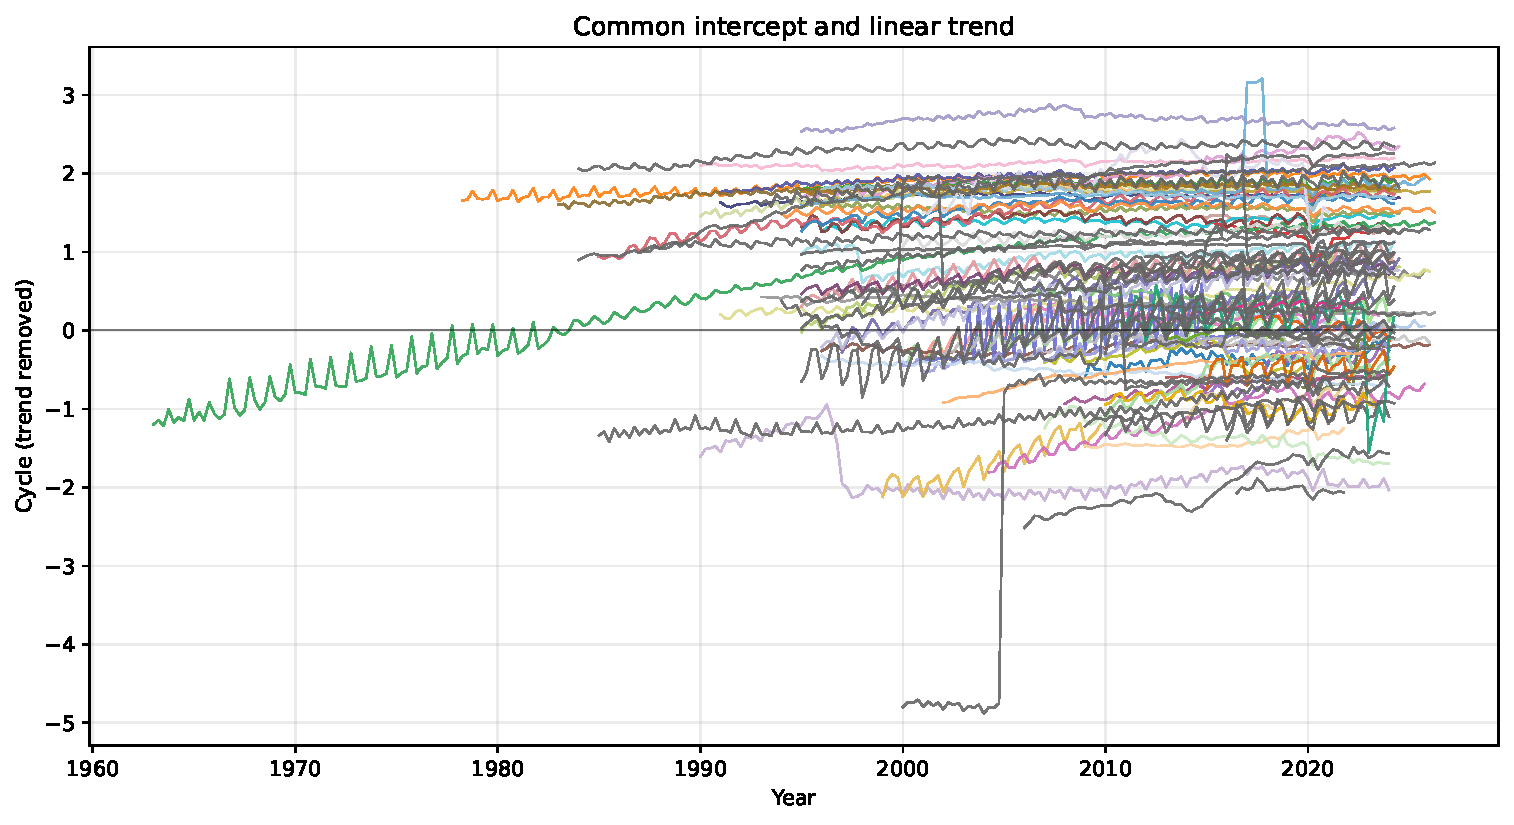
\includegraphics[width=0.75\textwidth]{figs/cycle_common_ag.pdf}
\caption{Country cycles after removing the linear trend.}
\end{figure}
\clearpage
\section{Random-effects intercepts, common linear trend}
2026-09-11 panel, full sample: log real GDP per worker. 95 countries, 8937 observations, 1963-Q1--2026-Q2. Fitted countries: 95. Observations: 8937. Log-likelihood: 11980.39. Ergodic mean of the cycle $E[z]=0.0940$ (0.0433).
Random intercepts $a_i\sim N(\alpha,\omega^2)$ with $\alpha=-6.3967$ (0.0411), $\omega=0.7246$ (0.0291). Posterior-mean $a_i$: mean -6.234, min -7.993, max -4.323. Common slope $g=0.0208$ (0.0009).
\begin{table}[h]
\centering
\caption{Regime AR(1), transition matrix, and ergodic $\pi$. Columns are regimes.}
\begin{tabular}{lccc}
\toprule
 & (0) & (1) & (2) \\
\midrule
$\mu$ & -0.1149 & 0.0000 & 0.3166 \\
 & (0.1171) & --- & (0.0684) \\ \addlinespace
$\sigma$ & 0.0867 & 0.2599 & 0.0376 \\
 & (0.0025) & (0.0105) & (0.0009) \\ \addlinespace
$\rho$ & 0.9898 & 0.0376 & 0.9899 \\
 & (0.0004) & (0.0622) & (0.0002) \\ \addlinespace
$\Pi_{0\cdot}$ & 0.9888 & 0.0047 & 0.0066 \\
 & (0.0024) & (0.0014) & (0.0019) \\ \addlinespace
$\Pi_{1\cdot}$ & 0.0268 & 0.9492 & 0.0239 \\
 & (0.0089) & (0.0102) & (0.0087) \\ \addlinespace
$\Pi_{2\cdot}$ & 0.0052 & 0.0029 & 0.9920 \\
 & (0.0015) & (0.0010) & (0.0015) \\ \addlinespace
$\pi$ & 0.4036 & 0.0671 & 0.5294 \\
 & (0.0422) & (0.0145) & (0.0438) \\ \addlinespace
\bottomrule
\end{tabular}
\end{table}
\begin{figure}[h]
\centering
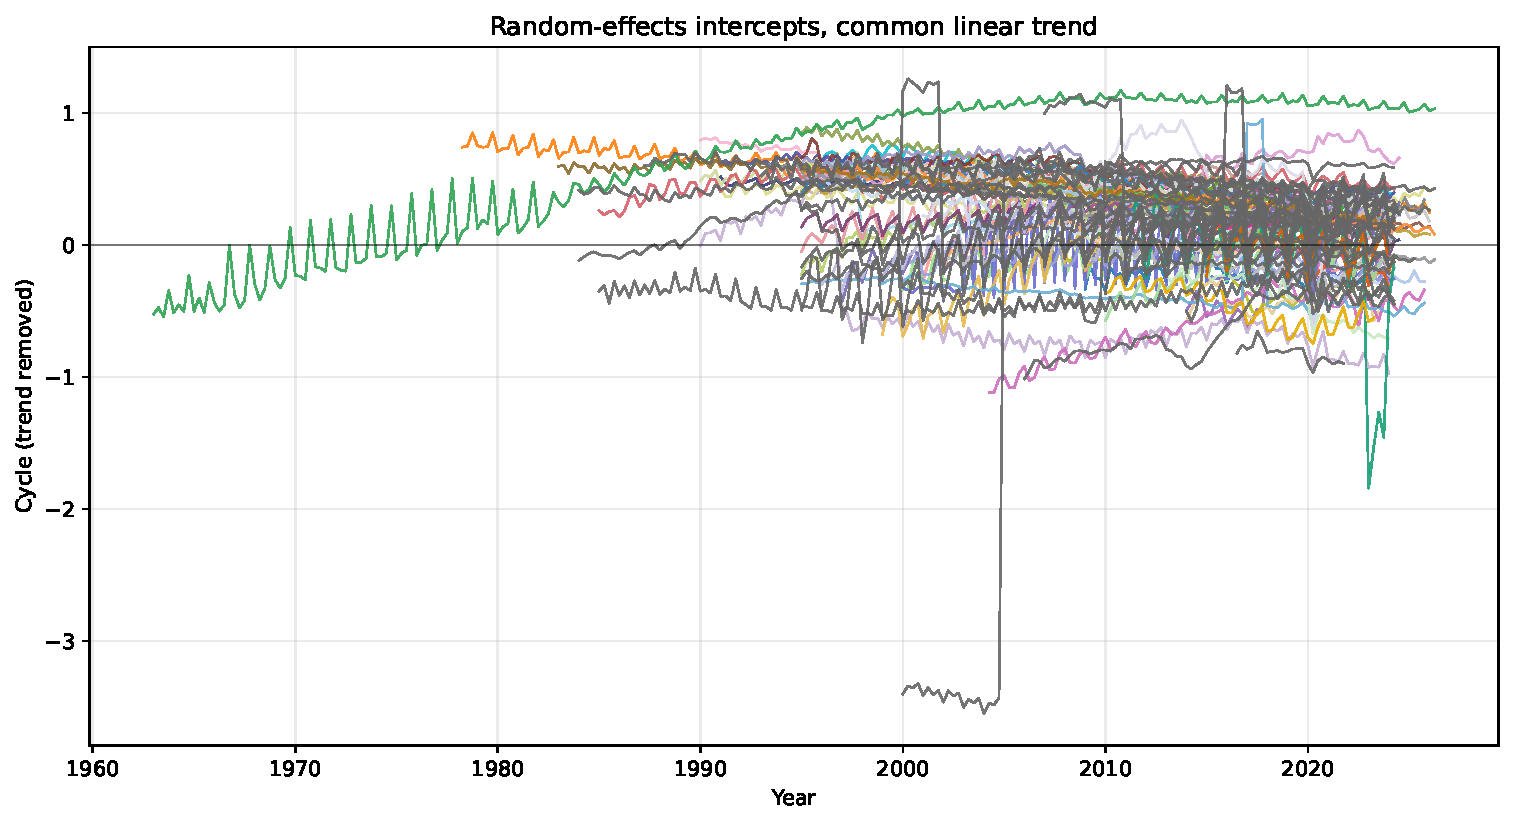
\includegraphics[width=0.75\textwidth]{figs/cycle_re_ai.pdf}
\caption{Country cycles after removing the linear trend.}
\end{figure}
\end{document}
